\documentclass[11pt]{article}

\usepackage[a4paper, margin=1in]{geometry}
\usepackage{amsmath, amssymb}
\usepackage{graphicx}
\usepackage{booktabs}
\usepackage{enumitem}
\usepackage{xcolor}
\usepackage{hyperref}
\hypersetup{colorlinks=true, linkcolor=blue, citecolor=blue, urlcolor=blue}

% Re-use macros from main paper
\newcommand{\Mzero}{\ensuremath{M_0}}
\newcommand{\Mphys}{\ensuremath{M_\text{phys}}}
\newcommand{\Mtl}{\ensuremath{M_\text{TL}}}
\newcommand{\Mtlphys}{\ensuremath{M_\text{TL+phys}}}
\newcommand{\Mrand}{\ensuremath{M_\text{rand}}}
\newcommand{\MAE}{\text{MAE}}

\renewcommand{\thesection}{S\arabic{section}}
\renewcommand{\thefigure}{S\arabic{figure}}
\renewcommand{\thetable}{S\arabic{table}}
\renewcommand{\theequation}{S\arabic{equation}}

\title{Supplementary Information for\\
\textit{Physics-Based Transfer Learning for Neural Network Surrogates of Metal--Insulator--Metal Absorbers}}
\author{Sang-Bae Choi$^{1,**}$, Joonhyub Kim$^{2,3}$, Chang-Mo Kang$^{2,3,*}$ \\[0.4em]
\small $^{1}$Independent Researcher, Busan 46264, Republic of Korea \\
\small $^{2}$Department of Nanomechatronics Engineering, Pusan National University, Busan 46241, Republic of Korea \\
\small $^{3}$School of Transdisciplinary Engineering, Pusan National University, Busan 46241, Republic of Korea \\[0.3em]
\small $^{*}$Corresponding author: \texttt{fd1kcm@pusan.ac.kr} \quad $^{**}$Co-corresponding author: \texttt{sbchoi129@gmail.com}}
\date{}

\begin{document}
\maketitle

\noindent
This document contains the full ablation tables, baseline comparisons, and supporting analyses referenced in the main text. The supplement comprises Sections~S1--S19 (S17, the TMM geometry-constraint sensitivity; S18, the Reviewer~\#2-requested figures; and S19, the correction change-log, were added in revision).

% ============================================================
\section{Random Pre-training Baseline (full table)}
\label{sec:si_random}
% ============================================================

To verify that transfer learning benefits arise from physics content rather than pre-training regularization effects, we compared $\Mtl$ against $\Mrand$ (pre-trained on uniformly random absorptance spectra). Table~\ref{tab:random} reports the full per-seed comparison.

\begin{table}[htbp]\centering\small
\caption{Random pre-training baseline ($\Mrand$) vs.\ physics-based models on Structure~A (mean $\pm$ std, 10 seeds). $\Mrand$ (pre-trained on uniformly random absorptance spectra with no physical content) is statistically indistinguishable from training from scratch ($\Mzero$), whereas TMM pre-training ($\Mtl$) reduces MAE by $20$--$50\%$, confirming that the PBTL benefit arises from genuine physics knowledge, not mere weight initialization or regularization.}
\label{tab:random}
\begin{tabular}{r ccc}\toprule
$n$ & $\Mzero$ & $\Mtl$ & $\Mrand$\\\midrule
50  & $8.87 \pm 1.01$ & $4.46 \pm 0.58$ & $8.79 \pm 1.03$\\
100 & $5.59 \pm 0.43$ & $3.26 \pm 0.19$ & $5.83 \pm 0.36$\\
200 & $3.63 \pm 0.30$ & $2.45 \pm 0.07$ & $3.83 \pm 0.15$\\
350 & $2.45 \pm 0.14$ & $1.97 \pm 0.03$ & $2.50 \pm 0.03$\\\bottomrule
\end{tabular}
\end{table}

The gap between $\Mtl$ and $\Mrand$ is $0.5$--$4.3$\,pp across training sizes (largest at small $n$), confirming that the TMM pre-training signal contains genuine physics knowledge that random initialization cannot replicate; $\Mrand$ itself tracks $\Mzero$ to within ${\sim}5\%$.


% ============================================================
\section{TMM Pre-training Data Size Sensitivity}
\label{sec:si_tmm_size}
% ============================================================

\begin{table}[htbp]\centering\small
\caption{Effect of TMM pre-training data size (Structure A, 3 seeds per condition).}
\label{tab:tmm_size}
\begin{tabular}{r rr c cc c}\toprule
$N_\text{TMM}$ & \textbf{Gen.} & \textbf{Pre-train} & \textbf{TMM val} & \multicolumn{2}{c}{\textbf{Fine-tuned MAE (\%)}} & \textbf{Overhead}\\
 & \textbf{(s)} & \textbf{(s)} & \textbf{MAE} & $n=100$ & $n=350$ & \textbf{(\%)}\\\midrule
Scratch & --- & --- & --- & $5.80 \pm 0.31$ & $2.35 \pm 0.09$ & ---\\
500     & 1.9  & 9   & 1.70\% & $4.30 \pm 0.16$ & $2.47 \pm 0.07$ & 0.1\%\\
1{,}000 & 3.8  & 18  & 1.59\% & $4.03 \pm 0.26$ & $2.33 \pm 0.06$ & 0.1\%\\
2{,}000 & 7.8  & 35  & 0.77\% & $3.57 \pm 0.16$ & $2.11 \pm 0.02$ & 0.3\%\\
5{,}000 & 18.9 & 88  & 0.45\% & $\mathbf{3.19 \pm 0.06}$ & $\mathbf{1.99 \pm 0.04}$ & 0.7\%\\\bottomrule
\end{tabular}
\end{table}

\textbf{Overhead} is computed as (TMM generation + pre-training time) / RCWA generation time for $500$ total samples (${\sim}15{,}000$\,s at ${\sim}30$\,s/sample on RTX 4070 Ti SUPER). The benefit increases monotonically with $N_\text{TMM}$ up to the largest size tested ($5{,}000$): the $\Mtl$-vs-$\Mzero$ improvement at $n=100$ grows from $+26\%$ ($500$) to $+45\%$ ($5{,}000$), with $N_\text{TMM}=2{,}000$ already capturing most of the gain ($+38\%$); even $500$ samples provide a $+26\%$ improvement at ${<}\,0.5\%$ overhead. Pre-training times are measured with the GPU full-batch implementation.


% ============================================================
\section{Learning Rate Ablation}
\label{sec:si_lr}
% ============================================================

A potential confound is that $\Mtl$ uses a lower fine-tuning learning rate ($3 \times 10^{-4}$) than $\Mzero$ ($10^{-3}$). We conducted a full factorial sweep ($2$ models $\times$ $2$ learning rates $\times$ $4$ data sizes $\times$ $3$ seeds $= 48$ runs).

\begin{table}[htbp]\centering\small
\caption{Learning-rate ablation across all three structures (3 seeds): $\Mtl$-vs-$\Mzero$ weight-transfer benefit (\%) at matched LR ($10^{-3}$, which controls the LR confound) and at the deployment fine-tuning LR ($3{\times}10^{-4}$).}
\label{tab:lr_ablation}
\begin{tabular}{ll cccc}\toprule
\textbf{Struct.} & \textbf{LR} & $n{=}50$ & $n{=}100$ & $n{=}200$ & $n{=}350$\\\midrule
A & $10^{-3}$          & $+38$ & $+40$ & $+29$ & $+16$\\
  & $3{\times}10^{-4}$ & $+53$ & $+52$ & $+46$ & $+34$\\\midrule
B & $10^{-3}$          & $+26$ & $+16$ & $+15$ & $+11$\\
  & $3{\times}10^{-4}$ & $+38$ & $+23$ & $+16$ & $+12$\\\midrule
C & $10^{-3}$          & $+8$  & $+2$  & $+4$  & $0$\\
      & $3{\times}10^{-4}$ & $+16$ & $+9$  & $+5$  & $+4$\\\bottomrule
\end{tabular}
\end{table}

At the matched learning rate ($10^{-3}$) the weight-transfer benefit stays clearly positive for Structures~A ($+16$ to $+40\%$) and~B ($+11$ to $+26\%$) and is marginal for the low-fidelity Structure~C (marginally negative to $+8\%$ at matched LR, dipping to ${\approx}-0.5\%$ at the largest pool), confirming that the benefit is \emph{not} an artifact of the lower fine-tuning rate used for transfer; the deployment rate ($3{\times}10^{-4}$) further improves it by better preserving the pre-trained features. The matched-LR benefit is graded by source fidelity ($A>B>C$), consistent with the fidelity-graded pattern of the main results. The Structure-C rows in this ablation use the isotropic single-output Structure-C variant, whose $\Mzero$ baseline differs from the main dual-polarization Structure-C, so they are not directly comparable to the $+9.7\%$ benefit of the main-text Structure-C table. These ablations use a training batch of $4{,}096$ for efficiency; because $\Mzero$ and $\Mtl$ are trained identically within each cell, the within-cell $\Mtl$-vs-$\Mzero$ contrast is not biased by the batch-size choice.


% ============================================================
\section{Architecture Ablation: ResNet vs.\ MLP}
\label{sec:si_arch}
% ============================================================

To rule out that physics features and TL primarily compensate for the ResNet backbone's capacity, we compare the ResNet-256-4 backbone ($566{,}529 \approx 567$\,K parameters) against a plain MLP without residual connections or LayerNorm (an input projection to $256$ followed by three $256$-unit hidden layers and a $128$-unit head, SiLU activations; $233{,}473 \approx 233$\,K parameters) under identical training protocols.

\begin{table}[htbp]\centering\small
\caption{Architecture ablation across all three structures (3 seeds): $\Mtl$-vs-$\Mzero$ benefit (\%) with the ResNet-256-4 backbone vs.\ a plain MLP (three $256$-unit hidden layers; Section~S4).}
\label{tab:arch_ablation}
\begin{tabular}{ll cccc}\toprule
\textbf{Struct.} & \textbf{Arch} & $n{=}50$ & $n{=}100$ & $n{=}200$ & $n{=}350$\\\midrule
A & ResNet & $+52$ & $+49$ & $+37$ & $+25$\\
  & MLP    & $+53$ & $+47$ & $+32$ & $+21$\\\midrule
B & ResNet & $+29$ & $+17$ & $+17$ & $+12$\\
  & MLP    & $+37$ & $+16$ & $-2$  & $-9$\\\midrule
C & ResNet & $+19$ & $+6$  & $-1$  & $-1$\\
      & MLP    & $+35$ & $+8$  & $-5$  & $-7$\\\bottomrule
\end{tabular}
\end{table}

This ablation uses the isotropic single-output Structure-C variant, whose $\Mzero$ baseline differs from the main dual-polarization Structure-C (the main-text Structure-C table), so its Structure-C cells are not directly comparable to the main $+9.7\%$ benefit. The ResNet backbone yields a robustly positive transfer benefit for Structures~A and~B and a marginal-to-neutral outcome for the lowest-fidelity Structure~C at the largest training sizes (Structure~A $+25$ to $+52\%$; Structure~B $+12$ to $+29\%$; Structure~C $-1$ to $+19\%$, dipping marginally negative with the ResNet, not only the MLP). With a plain MLP the benefit holds for the high-fidelity Structure~A but turns \emph{negative} at large~$n$ for Structures~B and~C ($-9\%$ and $-7\%$ at $n=350$), indicating that for moderate- and low-fidelity sources the residual/normalized ResNet architecture is needed for stable transfer. We report this architecture dependence as a robustness caveat: PBTL's benefit is not architecture-agnostic, and the residual backbone used throughout this work is the stable choice.


% ============================================================
\section{Permutation Feature Importance}
\label{sec:si_features}
% ============================================================

We quantify the contribution of each physics feature via permutation importance: for each of the $17$ features (Structure~A), we randomly shuffle its values ($10$ repetitions) while holding all other features fixed, and measure the resulting MAE increase.

\begin{table}[htbp]\centering\small
\caption{Top 10 physics features by permutation importance ($\Mphys$, Structure A, $n=350$).}
\label{tab:feature_importance}
\begin{tabular}{clcc}\toprule
\textbf{Rank} & \textbf{Feature} & \textbf{Category} & $\Delta$\textbf{MAE (\%)}\\\midrule
1 & $f_\text{rect} = W_x W_y / P^2$ & Fill fraction & $+8.88$\\
2 & $\cos(\varphi_{\text{SiO}_2})$ & Cavity resonance & $+5.24$\\
3 & $\sin(\varphi_{\text{SiO}_2})$ & Cavity resonance & $+3.90$\\
4 & $\sin(\varphi_{\text{TiO}_2})$ & Cavity resonance & $+3.71$\\
5 & $t_1/\delta$ & Skin depth ratio & $+3.54$\\
6 & $P/\lambda$ & Sub-wavelength & $+2.41$\\
7 & $W_y/W_x$ & Geometry & $+2.08$\\
8 & $t_\text{mid}/\delta$ & Skin depth ratio & $+1.90$\\
9 & $\alpha_\text{metal}$ & Geometry & $+1.51$\\
10 & $\cos(\varphi_{\text{TiO}_2})$ & Cavity resonance & $+1.36$\\
\end{tabular}
\end{table}

\begin{table}[htbp]\centering\small
\caption{Category-level aggregation of permutation feature importance ($\Mphys$, Structure~A, $n=350$). Cavity resonance and fill fraction together account for ${\sim}60\%$ of total importance.}
\label{tab:category_importance}
\begin{tabular}{lccc}\toprule
\textbf{Category} & \textbf{Features} & $\Mphys$ \textbf{Total} & \textbf{\% of Total}\\\midrule
Cavity Resonance     & 4 & $+14.21\%$ & \textbf{37\%}\\
Fill Fraction        & 2 & $+9.03\%$  & \textbf{23\%}\\
Skin Depth Ratio     & 3 & $+5.78\%$  & 15\%\\
Angle \& Geometry    & 3 & $+4.62\%$  & 12\%\\
Sub-wavelength Ratio & 3 & $+4.11\%$  & 11\%\\
Optical Path         & 2 & $+0.72\%$  & $<2\%$\\
\end{tabular}
\end{table}

Feature importance rankings are nearly identical between $\Mphys$ and $\Mtlphys$, confirming that feature utility is independent of whether transfer learning was applied.


% ============================================================
\section{TMM-as-Input Baseline}
\label{sec:si_tmm_input}
% ============================================================

An alternative to encoding TMM knowledge through weight initialization (PBTL) is to supply the TMM prediction directly as an additional input feature: $M_\text{TMM-in}$ appends the scalar $A_\text{TMM}(\mathbf{x}, \lambda)$ to the geometry input and trains from scratch.

\begin{table}[htbp]\centering\small
\caption{TMM-as-input baseline vs.\ PBTL variants (Structure A, 5 seeds).}
\label{tab:tmm_input}
\begin{tabular}{r cccc}\toprule
$n$ & $\Mzero$ & $M_\text{TMM-in}$ & $\Mphys$ & $\Mtlphys$\\\midrule
50  & $8.28 \pm 0.50$ & $7.39 \pm 0.67$ & $7.21 \pm 0.67$  & $\mathbf{4.31 \pm 0.34}$\\
100 & $5.60 \pm 0.39$ & $5.60 \pm 0.18$ & $5.29 \pm 0.40$  & $\mathbf{3.20 \pm 0.24}$\\
200 & $3.54 \pm 0.17$ & $3.79 \pm 0.42$ & $3.59 \pm 0.10$  & $\mathbf{2.43 \pm 0.11}$\\
350 & $2.45 \pm 0.22$ & $2.46 \pm 0.12$ & $2.64 \pm 0.06$  & $\mathbf{1.89 \pm 0.02}$\\\bottomrule
\end{tabular}
\end{table}

$M_\text{TMM-in}$ provides only marginal improvement---$+10.7\%$ over $\Mzero$ at $n{=}50$, then neutral-to-negative ($-0.1\%$, $-7.0\%$, $-0.6\%$ at $n{=}100,200,350$)---whereas weight-level transfer with physics features ($\Mtlphys$) is the best model at every size, confirming that distributed weight-level transfer extracts more from the same TMM physics than direct input concatenation.


% ============================================================
\section{Multi-fidelity Baseline Comparison}
\label{sec:si_mf}
% ============================================================

We compare PBTL against four multi-fidelity baselines: (1)~linear correction, (2)~residual NN, (3)~Co-Kriging (Kennedy \& O'Hagan autoregressive model), and (4)~Co-Kriging with physics features. All baselines use $500$ TMM samples and $50$--$350$ RCWA fine-tuning samples.

\begin{table}[htbp]\centering\small
\caption{Multi-fidelity baseline comparison (Structure A, 5 seeds, 4 training sizes).}
\label{tab:multifidelity_baselines}
\begin{tabular}{r ccccc c}\toprule
$n$ & $\Mzero$ & Linear & ResNN & Co-Krig & Co-Krig+phys & $\Mtlphys$ (ours)\\\midrule
50  & $8.25 \pm 0.51$ & $7.55 \pm 0.08$ & $7.83 \pm 0.69$ & $7.41 \pm 0.35$ & $7.08 \pm 0.32$ & $\mathbf{4.36 \pm 0.29}$\\
100 & $5.70 \pm 0.30$ & $7.49 \pm 0.10$ & $4.77 \pm 0.21$ & $6.67 \pm 0.14$ & $6.08 \pm 0.28$ & $\mathbf{3.07 \pm 0.24}$\\
200 & $3.89 \pm 0.38$ & $7.47 \pm 0.04$ & $3.46 \pm 0.04$ & $5.89 \pm 0.17$ & $4.82 \pm 0.30$ & $\mathbf{2.21 \pm 0.05}$\\
350 & $2.58 \pm 0.04$ & $7.42 \pm 0.01$ & $2.45 \pm 0.15$ & $5.13 \pm 0.05$ & $3.93 \pm 0.12$ & $\mathbf{1.77 \pm 0.03}$\\\bottomrule
\end{tabular}
\end{table}

\subsection*{Sparse Co-Kriging with Expanded TMM Budget}

A natural concern is whether Co-Kriging would catch up if given PBTL's $5{,}000$-sample TMM budget. Cubic Gaussian-process (GP) scaling makes a dense fit on $2{,}000+$ samples impractical at this budget in our implementation. We therefore replaced each per-wavelength GP with a sparse variational GP (SVGP, $M=128$ inducing points, $k$-means initialization).

\begin{table}[htbp]\centering\small
\caption{Sparse SVGP Co-Kriging with expanded TMM budget (Structure A, $M=128$ inducing points, 3 seeds).}
\label{tab:sparse_cokriging}
\begin{tabular}{r ccc c}\toprule
$n_\text{RCWA}$ & Sparse $N_\text{TMM}=500$ & Sparse $N_\text{TMM}=2{,}000$ & Dense $N_\text{TMM}=500$ (ref.) & $\Mtlphys$\\\midrule
100 & $10.11 \pm 0.52$ & $9.96 \pm 0.59$ & $11.33 \pm 0.96$ & $\mathbf{7.58 \pm 0.33}$\\
350 & $9.24 \pm 0.42$  & $9.04 \pm 0.65$ & $7.69 \pm 0.31$  & $\mathbf{4.85 \pm 0.13}$\\\bottomrule
\end{tabular}
\end{table}

Quadrupling the TMM budget closes only $0.15$--$0.20$\,pp of the gap to PBTL, ruling out a data-budget asymmetry.

\subsection*{Deep Composite Multi-Fidelity NN}

We additionally implemented the deep composite architecture of Meng \textit{et al.}: a low-fidelity (LF) ResNet pretrained on $5{,}000$ TMM samples is frozen, and a high-fidelity (HF) head predicts $y_H = \alpha(\lambda)y_L + \beta(\lambda) + F_\text{NL}(x, \lambda, y_L)$. The LF information enters at the output level rather than the weight level. The deep multi-fidelity neural network (MF-NN) achieves $7.18/5.24/3.48/2.59\%$ MAE at $n=50/100/200/350$ ($3$ seeds), leaving a $32$--$41\%$ relative gap to $\Mtlphys$.

\subsection*{Co-Kriging Kernel Sensitivity}

To rule out kernel-selection bias, we swept four kernel families and two input configurations ($3$ seeds): Mat\'{e}rn-$5/2$ tight, Mat\'{e}rn-$5/2$ wide, Mat\'{e}rn-$3/2$, RBF, and Mat\'{e}rn-$5/2$+phys. The best variant (Mat\'{e}rn-$5/2$+phys) reaches $12.52/10.14/8.65/7.68\%$ MAE---a $0.1$--$0.6$\,pp improvement over the tight Mat\'{e}rn-$5/2$ but still $37$--$58\%$ worse than $\Mtlphys$. RBF performs substantially worse ($11.7$--$14.3\%$) because infinite smoothness is inappropriate for non-smooth cavity resonance features. (This kernel-sensitivity sweep was run on the earlier visible-band Structure-A pipeline and was not regenerated on the corrected pipeline; it is reported only as a kernel-family ranking, in which every Co-Kriging kernel remained well behind $\Mtlphys$.)


% ============================================================
\section{Architecture Sensitivity: Per-Wavelength vs.\ Full-Spectrum}
\label{sec:si_fs}
% ============================================================

We re-ran $\Mzero$ and $\Mtl$ with a Full-Spectrum (FS) ResNet whose output is the entire $100$-wavelength absorptance vector at once: input is $\text{norm}(\mathbf{x})$ (no wavelength index), the backbone is identical, and the head is replaced by a single linear layer $\mathbb{R}^{256} \rightarrow \mathbb{R}^{100}$. Pre-training uses the same $5{,}000$-sample TMM library, and fine-tuning uses the same fixed RCWA split; the Full-Spectrum ablation is run over $3$ seeds.

\begin{table}[htbp]\centering\small
\caption{Architecture sensitivity: per-wavelength vs.\ Full-Spectrum (FS) ResNet (Structure A). The per-wavelength columns reproduce the main-text $10$-seed Structure-A result; the Full-Spectrum columns are a $3$-seed ablation trained on the same fixed split.}
\label{tab:fs_arch}
\begin{tabular}{r cc cc}\toprule
& \multicolumn{2}{c}{\textbf{Full-Spectrum (FS)}} & \multicolumn{2}{c}{\textbf{Per-wavelength}}\\
\cmidrule(lr){2-3}\cmidrule(lr){4-5}
$n$ & $\Mzero^\text{FS}$ & $\Mtl^\text{FS}$ & $\Mzero$ & $\Mtl$\\\midrule
50  & $9.46 \pm 1.12$ & $4.92 \pm 0.32$ & $\mathbf{8.36 \pm 0.63}$ & $\mathbf{4.21 \pm 0.49}$\\
100 & $6.29 \pm 0.07$ & $3.87 \pm 0.06$ & $\mathbf{5.68 \pm 0.33}$ & $\mathbf{3.11 \pm 0.17}$\\
200 & $4.54 \pm 0.16$ & $3.04 \pm 0.12$ & $\mathbf{3.93 \pm 0.35}$ & $\mathbf{2.39 \pm 0.11}$\\
350 & $3.33 \pm 0.12$ & $2.51 \pm 0.02$ & $\mathbf{2.64 \pm 0.09}$ & $\mathbf{1.82 \pm 0.07}$\\\bottomrule
\end{tabular}
\end{table}

The per-wavelength architecture outperforms FS at every training size: across both $\Mzero$ and $\Mtl$ and all four training sizes, the FS MAE is $11$--$38\%$ higher than the per-wavelength MAE (per-cell relative gap $(\MAE_\text{FS}-\MAE_\text{PW})/\MAE_\text{PW}$, with the per-wavelength baseline taken from the main-text $10$-seed result). PBTL pre-training nonetheless still delivers a substantial relative TL benefit on FS ($+24.6\%$ to $+48.0\%$). Thus the weight-transfer effect is not unique to the per-wavelength output formulation, although the backbone ablation in Supplementary Section~S4 shows that the benefit is not fully architecture-agnostic.


% ============================================================
\section{Material Generalization: Au + Structure B}
\label{sec:si_au_b}
% ============================================================

To test whether the Cr-vs-Au comparison generalizes beyond Structure~A, we additionally ran the 4-way protocol on Structure~B using corrected Johnson--Christy Au optical constants ($500$ targeted Au RCWA samples, $499$ finite and $419$ reliable after the documented physicality filter ($A\in[-0.005,1.005]$ at every wavelength, after which $A$ and $R$ are clipped to $[0,1]$), $2{,}000$ Au TMM pre-training samples, $5$ seeds per condition; the larger Au-B discard than Au-A reflects gold's stronger oblique-incidence grazing-order sensitivity, Supplementary Section~S16). After reserving $40$ test and $40$ validation samples, the training pool contains $339$ Au RCWA samples. The Au Structure-B experiment uses gold's native visible band ($380$--$780$\,nm), where its plasmonic resonance lies, so it probes \emph{material} rather than band generalization.

\begin{table}[htbp]\centering\small
\caption{Corrected 4-way model comparison on Au/SiO$_2$ Structure~B (mean $\pm$ std, 5 seeds) on gold's visible band ($380$--$780$\,nm). \emph{TL benefit} is the marginal effect of weight-level transfer alone, $(1 - \MAE_{\Mtl}/\MAE_{\Mzero}) \times 100\%$ ($\Mtl$ vs.\ $\Mzero$, both \emph{without} physics features). On the corrected data the benefit is positive at every training size.}
\label{tab:material_gen_B}
\begin{tabular}{r cccc r}\toprule
$n$ & $\Mzero^\text{Au,B}$ & $\Mphys^\text{Au,B}$ & $\Mtl^\text{Au,B}$ & $\Mtlphys^\text{Au,B}$ & TL benefit ($\Mtl$ vs.\ $\Mzero$)\\\midrule
50  & $10.48 \pm 0.68$ & $10.17 \pm 0.88$ & $\mathbf{7.54 \pm 0.30}$ & $7.57 \pm 0.33$ & $+28.0\%$\\
100 & $8.24 \pm 0.31$  & $7.87 \pm 0.34$  & $\mathbf{6.90 \pm 0.42}$ & $6.93 \pm 0.27$ & $+16.4\%$\\
200 & $6.97 \pm 0.32$  & $6.81 \pm 0.23$  & $6.45 \pm 0.21$ & $\mathbf{6.33 \pm 0.24}$ & $+7.5\%$\\
339 & $6.06 \pm 0.11$  & $6.20 \pm 0.23$  & $5.78 \pm 0.08$ & $\mathbf{5.73 \pm 0.10}$ & $+4.6\%$\\\bottomrule
\end{tabular}
\end{table}

On the corrected Au--B data, weight-level transfer ($\Mtl$ vs.\ $\Mzero$) is positive at every training size---$+28.0\%$ at $n=50$, $+16.4\%$ at $n=100$, $+7.5\%$ at $n=200$, and $+4.6\%$ at the saturated pool ($n=339$)---weaker than Au Structure~A but, unlike the earlier pre-correction visible-band check (which had turned slightly negative at the largest pool), no longer negative. Unlike Structure~A, the explicit physics features give only a small standalone gain that reverses at the largest pool ($\Mphys$ within ${\sim}0.4$\,pp of $\Mzero$---the planar EMA poorly captures the ring--disk Fano coupling), and the combined model satisfies $\Mtlphys \approx \Mtl$; the benefit therefore comes almost entirely from weight-level transfer. The corrected TMM--RCWA fidelity is median $r=0.78$, median MAE $=15.4\%$. We report this as a single descriptive cross-material result and do not draw a cross-structure mechanistic conclusion from it. Both Au checks (Structures~A and~B) use the deployment learning rates (scratch lr~$=10^{-3}$, transfer lr~$=3\times10^{-4}$); the matched-learning-rate control that rules out a learning-rate artifact (Section~S3) was performed for the three primary Cr structures and is not repeated for these secondary cross-material checks.


% ============================================================
\section{Per-Seed Results for Structure A at n=350, 10 seeds}
\label{sec:si_per_seed}
% ============================================================

\begin{table}[htbp]\centering\footnotesize
\caption{Per-seed test MAE (\%) for Structure A at $n=350$ (10 seeds).}
\label{tab:per_seed_a}
\begin{tabular}{r cccc}\toprule
\textbf{Seed} & $\Mzero$ & $\Mphys$ & $\Mtl$ & $\Mtlphys$\\\midrule
42  & 2.63 & 2.53 & 1.77 & 1.72\\
123 & 2.52 & 2.64 & 1.79 & 1.76\\
777 & 2.54 & 2.48 & 1.88 & 1.74\\
321 & 2.62 & 2.44 & 1.73 & 1.81\\
456 & 2.58 & 2.63 & 1.78 & 1.81\\
654 & 2.59 & 2.57 & 1.92 & 1.87\\
999 & 2.69 & 2.42 & 1.85 & 1.80\\
111 & 2.66 & 2.53 & 1.73 & 1.81\\
222 & 2.76 & 2.52 & 1.91 & 1.82\\
333 & 2.84 & 2.43 & 1.80 & 1.80\\
\midrule
\textbf{Mean} & 2.64 & 2.52 & 1.82 & \textbf{1.79}\\
\textbf{Std}  & 0.09 & 0.07 & 0.07 & 0.04\\\bottomrule
\end{tabular}
\end{table}


% ============================================================
\section{Structure C: Anisotropic TMM Pre-training Details}
\label{sec:si_struct_c}
% ============================================================

Structure~C is inherently dual-polarization, requiring separate TE and TM absorptance predictions. We use an anisotropic TMM variant (\texttt{tmm\_struct\_c\_aniso}) that computes separate TE and TM absorptance spectra, with $\varepsilon_\text{eff}^\text{TE}$ built from $f_y = W_y/P$ and $\varepsilon_\text{eff}^\text{TM}$ from $f_x = W_x/P$ (the anisotropic-EMA equation of the main text). Five additional polarization-specific features are included: (1)~the directional fill fraction $f_x = W_x/P$, (2)~the directional fill fraction $f_y = W_y/P$, (3)~the normalized geometric anisotropy $|f_x - f_y|/(f_x + f_y)$, and the polarization-resolved sub-wavelength resonance ratios (4)~$W_x^2/(P\lambda)$ and (5)~$W_y^2/(P\lambda)$. The total physics feature count is 18 (13 base + 5 polarization).

The dual-polarization architecture places two independent sigmoid heads on the shared 256-dimensional representation, predicting $R_\text{TE}$ and $R_\text{TM}$; absorptances are derived deterministically as
\[
A_\text{TE} = 1 - R_\text{TE}, \qquad A_\text{TM} = 1 - R_\text{TM},
\]
and transmittance is negligible (Section~S12) and not predicted. The training loss is the sum of the four per-channel MSE terms on $(A_\text{TE}, R_\text{TE}, A_\text{TM}, R_\text{TM})$.


% ============================================================
\section{Transmittance Validation}
\label{sec:si_transmittance}
% ============================================================

\begin{table}[htbp]\centering\small
\caption{Transmittance statistics from RCWA simulations across all three MIM structures (reliable-sample subset), confirming that the Cr ground mirror keeps transmittance small: per-structure $T_\text{mean} < 1\%$ and $T_\text{max} \lesssim 2.3\%$, so the structures operate as near-opaque absorbers. The RCWA training labels are the full absorptance $A = 1 - R - T$; because the surrogate predicts $R$ and outputs $A = 1 - R$, this residual transmittance bounds the absorptance-output approximation error---at most $T$ per sample (mean ${\sim}0.1$--$0.6\%$, up to ${\sim}2.3\%$ worst-case), as quantified in the main-text Neural Network Architecture section---small relative to the reported MAE at small and medium training pools though not negligible against the smallest MAE values at the largest pools.}
\label{tab:transmittance}
\begin{tabular}{lccc}\toprule
\textbf{MIM Structure} & $T_\text{mean}$ & $T_\text{max}$ & \textbf{\% with $T < 0.01$}\\\midrule
A (Dual-Cavity)  & 0.0013 & 0.0142 & 99.5\%\\
B (Ring-Disk)    & 0.0061 & 0.0209 & 71.6\%\\
C-TE (Dual-Pol)  & 0.0046 & 0.0224 & 83.0\%\\
C-TM (Dual-Pol)  & 0.0054 & 0.0234 & 78.5\%\\\bottomrule
\end{tabular}
\end{table}


% ============================================================
\section{Preliminary Inverse Design Investigation}
\label{sec:si_inverse}
% ============================================================

We attempted inverse design using the trained PBTL surrogate ($\Mtlphys$, Structure~A) with gradient-based optimization. This probe was run on the earlier visible-band ($380$--$780$\,nm, fixed $N{=}5$) surrogate and is reported as a qualitative, preliminary demonstration; the adversarial-gradient failure mode it illustrates is reported as an illustrative example on that superseded visible-band surrogate and was not revalidated on the corrected pipeline. Both RCWA solvers showed significant validation failures:

\begin{table}[htbp]\centering\small
\caption{Inverse design validation failure analysis.}
\label{tab:inverse_design}
\begin{tabular}{llcl}\toprule
\textbf{Solver} & \textbf{Result} & \textbf{MAE} & \textbf{Root Cause}\\\midrule
torcwa          & Complete failure   & $A \approx 0$  & Adversarial exploitation of surrogate gradient\\
grcwa           & High error         & 24--41\%       & Solver parameter mismatch + extrapolation\\
grcwa (sanity)  & Failed reproduction & 12.22\%        & Fundamental solver incompatibility\\\bottomrule
\end{tabular}
\end{table}

These failures reflect extrapolation limits of the surrogate model and fundamental incompatibilities between RCWA solver implementations. The cross-solver discrepancy is confined to the inverse design context; it does not affect the forward modeling results, which use only torcwa for both training and evaluation within the design space. Future work should employ physics-informed inverse methods with constrained optimization to prevent adversarial exploitation of surrogate gradients.


% ============================================================
\section{Sub-band TMM--RCWA Fidelity Decomposition for Structures B and C}
\label{sec:si_subband}
% ============================================================

To support the wavelength-region-dependent fidelity interpretation in
the cross-structure analysis of the main text and the Structure-B
characterization there, we decompose the corrected TMM--RCWA fidelity
of Structures B and C into spectral sub-bands. The same 500-sample
RCWA/TMM pairs used for the main-text TMM--RCWA fidelity table are partitioned by
wavelength, and per-sample Pearson correlation $r$ and absolute MAE are
recomputed restricted to each sub-band; the structures' full operating
band (400--1800\,nm) is also reported for reference.

\begin{table}[htbp]\centering\small
\caption{Sub-band TMM--RCWA fidelity for Structures B and C (each on
the broadband 400--1800\,nm native grid; up to 500 samples per structure ($500$/$499$/$500$ for A/B/C)).
Median Pearson $r$ and median absolute MAE are reported per sub-band.
The deep-NIR rows isolate the sub-wavelength regime where the EMA
approximation underlying TMM is expected to be most accurate, while
the visible/short-wavelength rows isolate the region where Fano coupling
(Structure B) and polarization-resonance splitting (Structure C) are
strongest. The Full-broadband row reports the per-sample \emph{median} MAE and matches
the median values reported in the main-text TMM--RCWA fidelity table.}
\label{tab:subband_fidelity}
\begin{tabular}{lcccc}\toprule
\textbf{Sub-band} & \textbf{B median $r$} & \textbf{B median MAE} & \textbf{C median $r$} & \textbf{C median MAE}\\\midrule
Full broadband (400--1800\,nm) & $+0.96$ & $8.9\%$ & $+0.65$ & $16.9\%$\\
Visible (400--780\,nm) & $+0.95$ & $8.2\%$ & $+0.62$ & $12.5\%$\\
NIR-short (780--1200\,nm) & $+0.97$ & $9.7\%$ & $+0.64$ & $17.3\%$\\
NIR-long (1200--1800\,nm) & $\mathbf{+1.00}$ & $8.9\%$ & $+0.71$ & $18.4\%$\\
Deep NIR (1000--1800\,nm) & $+0.99$ & $9.0\%$ & $+0.63$ & $18.2\%$\\\bottomrule
\end{tabular}
\end{table}

\textbf{Interpretation.} On the corrected materials and grid, Structure~B
shows \emph{uniformly high} TMM--RCWA agreement: the median $r$ is
$0.95$--$1.00$ in every sub-band and the median MAE stays within
$\sim 8$--$10\%$ throughout. The earlier, apparent visible-band
``shape degradation'' was an artifact of the uncorrected optical constants;
with the corrected Johnson \& Christy data the EMA-based TMM tracks the shape of
Structure~B's spectra across the whole operating band, with an operating-band MAE
of $\sim 8$--$10\%$, consistent with Structure~B showing a positive
weight-transfer benefit (main-text Structure-B/C results). Structure~C is moderate
across all sub-bands (median $r \approx 0.62$--$0.71$, MAE
$\approx 12$--$18\%$); its lower overall fidelity---driven by the incomplete
polarization splitting of a planar EMA source---is consistent with its being
the smallest-benefit structure.

These sub-band measurements support the revised main-text narrative: the
cross-structure benefit ordering follows the absolute operating-band MAE
(A $<$ B $<$ C) rather than shape correlation $r$ alone, and Structure~B in
particular is now a \emph{high-fidelity} source in every sub-band rather than
a visible-band failure case (main-text cross-structure analysis and guidelines).

\textbf{Common operating band.} In the submitted version Structure~A was
simulated on a visible 380--780\,nm grid while Structures~B and~C used
400--1800\,nm, raising a visible-versus-broadband fairness question. In the
revised pipeline Structure~A is unified to the same 400--1800\,nm band as B
and C (Methods), so all three structures are now compared on a common
broadband grid and that asymmetry no longer applies; the visible
(400--780\,nm) sub-band cut above (B $+0.95/8.2\%$, C $+0.62/12.5\%$) is
reported for completeness, supporting the joint $r$-and-MAE diagnostic
recommended in the main-text practical-guidelines discussion.


% ============================================================
\section{Head-to-Head with Peng et al.'s PCA-Centroid Indicator}
\label{sec:si_peng}
% ============================================================

Reviewer point M8 asks for a direct comparison with the PCA-projected far-field
centroid distance proposed by Peng et al.\ (main-text reference). We
implemented their indicator on our own data: for each condition we fit PCA on the
pooled (TMM, RCWA) absorptance spectra and take the Euclidean distance between the
TMM and RCWA cluster centroids in the principal-component space (95\% variance
retained), and we benchmark it against our joint pilot-set $r$-and-MAE diagnostic
as a predictor of the measured weight-level transfer benefit. The benchmark spans
nine conditions: the three Cr structures and the six controlled noise-injection
levels on Structure~A (the noise-injection experiment of the main text).

\begin{table}[htbp]\centering\small
\caption{Per-condition values for the head-to-head. ``Peng dist.'' is the
PCA-centroid distance (95\% variance); ``our $r$'' is the median per-sample
TMM--RCWA shape correlation (the same statistic used in the main-text noise
table); ``benefit'' is the $\Mtl$-vs-$\Mzero$
weight-transfer benefit at $n=50$.}
\label{tab:peng_headtohead}
\begin{tabular}{lcccc}\toprule
\textbf{Condition} & \textbf{Peng dist.} & \textbf{our $r$} & \textbf{our MAE (\%)} & \textbf{benefit (\%)}\\\midrule
A (Structure)            & 0.74 & $+0.83$ & 7.9  & $+49.7$\\
B (Structure)            & 0.38 & $+0.96$ & 8.9  & $+36.3$\\
C (Structure)            & 1.62 & $+0.65$ & 16.9 & $+35.8$\\
noise $\sigma=0.00$      & 0.85 & $+0.77$ & 7.4  & $+47.3$\\
noise $\sigma=0.05$      & 0.86 & $+0.50$ & 8.0  & $+40.8$\\
noise $\sigma=0.10$      & 0.88 & $+0.35$ & 10.8 & $+33.0$\\
noise $\sigma=0.15$      & 0.92 & $+0.26$ & 14.0 & $+32.3$\\
noise $\sigma=0.20$      & 0.98 & $+0.21$ & 16.7 & $+22.6$\\
random ($\sigma=\infty$) & 2.52 & $-0.03$ & 33.0 & $-57.9$\\\bottomrule
\end{tabular}
\end{table}

\begin{table}[htbp]\centering\small
\caption{Predictive power (Pearson correlation with benefit) of each indicator,
on the three structures, the six noise levels, and all nine conditions. Lower
(more negative) is a stronger predictor for the distance/MAE; positive for $r$.
The shape-correlation $r$ here is the median per-sample statistic (consistent
with the main-text noise table), not the raw spectrum-level $r$.}
\label{tab:peng_corr}
\begin{tabular}{lccc}\toprule
\textbf{Predictor} & \textbf{3 structures} & \textbf{6 noise} & \textbf{all 9}\\\midrule
Peng centroid distance & $-0.26$ & $-0.99$ & $-0.86$\\
our MAE (amplitude)    & $\mathbf{-0.61}$ & $\mathbf{-0.98}$ & $\mathbf{-0.95}$\\
our $r$ (shape)        & $+0.12$ & $+0.81$ & $+0.73$\\\bottomrule
\end{tabular}
\end{table}

The operating-band \emph{absolute MAE} is the strongest single predictor of the
weight-transfer benefit across all nine conditions ($|r|=0.95$; rank correlation
$-1.0$ across the three structures), ahead of both the Peng centroid distance
($|r|=0.86$ for the published raw, $95\%$-variance definition; the strongest of the four Peng PCA variants we evaluated reaches $|r|\approx0.93$, still below the MAE's $0.95$) and the median per-sample shape correlation $r$ alone
($|r|=0.73$ combined). The amplitude--shape separation is sharpest on the controlled
noise sweep: there the MAE attains $|r|=0.98$ while the median shape-$r$ reaches only
$|r|=0.81$, even though the underlying sweep is monotone in fidelity (all three
predictors hold rank correlation $|\rho|=1$). The rank agreement confirms that each
indicator is a correctly-signed monotone marker, but the linear gap shows that the
benefit scales with the amplitude error far more tightly than with the shape
correlation. The discriminating regime is the three real structures, where the MAE
ordering matches the benefit ordering exactly (rank correlation $-1.0$) while both
the Peng distance and the shape-$r$ under-rank them ($B>A>C$ rather than $A>B>C$). The
three-structure \emph{linear} (Pearson) correlation is modest for every predictor at
this small training size---at $n=50$ all three structures, including the lower-fidelity
Structure~C, receive large transfer gains, compressing the amplitude--benefit spread---so
we read the three-structure result through its rank ordering (where MAE alone is monotone,
$\rho=-1.0$) rather than the three-point Pearson coefficient ($|r|=0.61$ for MAE,
$0.26$/$0.12$ for the Peng distance/shape-$r$); the linear amplitude--benefit gap is
established instead by the controlled six-level noise sweep ($|r|=0.98$ vs.\ $0.81$) and the
all-nine aggregate ($|r|=0.95$). We
emphasize that the Peng distance is a valid, correctly-signed monotone indicator;
the difference is that our amplitude (MAE) component is the stronger ordering signal in
this cross-fidelity, amplitude-dominated regime, and our diagnostic additionally
requires neither a PCA projection nor a pre-trained model. The comparison is
illustrative at $N=3$ structures and descriptive throughout (no significance is
claimed).


% ============================================================
\section{RCWA Fourier-Truncation Convergence}
\label{sec:si_convergence}
% ============================================================

Reviewer point M7 notes that the RCWA forward simulations were run at a fixed,
modest Fourier-truncation order and that the resulting truncation error was
absorbed into the reported surrogate MAE. To quantify this and to justify the
settings used for the regenerated dataset, we performed a per-(geometry,
wavelength) convergence study, sweeping the truncation order
$N\in\{5,9,13,17\}$ (the number of retained Fourier harmonics per in-plane
direction) and tracking the absolute absorptance. For the periodic
two-dimensional Structure-C geometries we resolve the two linear polarizations
separately (TE and TM); for Structures~A and B we report the unpolarized
absorptance.

The headline finding is that $N=5$---the order used in the original
submission---is under-converged, and the residual truncation error is
structure-dependent. Comparing $N=5$ against the converged $N=17$ reference,
the absolute-absorptance difference is $\approx 2.1$\,pp for Structure~A
(up to ${\sim}5.7$\,pp at long wavelengths), $\approx 3.4$\,pp for Structure~B,
and $\approx 5.5$\,pp for Structure~C on the TE channel, growing to as much as
${\sim}15$\,pp at long wavelengths ($\lambda \approx 1000$\,nm), where the
high-aspect-ratio anisotropic grating profile of Structure~C requires the most
harmonics to resolve. The TM channel of Structure~C is comparatively benign
($\lesssim 1$\,pp at the canonical geometry). Representative
$(\text{structure},\lambda)$ pairs are given in
Table~\ref{tab:si_convergence}.

This accuracy comes at a steep cost. The per-(geometry, wavelength) wall-clock
time grows from $\approx 0.4$\,s at $N=5$ to $\approx 28$\,s at $N=17$
(roughly a $70\times$ increase), and the peak memory grows from
$\approx 77$\,MB to $\approx 7$\,GB over the same range. The dataset
regeneration therefore uses \emph{per-wavelength adaptive} Fourier orders, up
to $N=17$, raised by a heuristic based on feature size and anisotropy rather
than held at a single fixed order: short wavelengths and the low-anisotropy
control geometries are assigned lower $N$, while the long-wavelength,
high-aspect-ratio Structure-C geometries are pushed to the maximum order
($N=17$, the practical memory ceiling), at which a small residual truncation can
persist. As a result, the surrogate MAE reported in the main text is dominated
by the network's approximation error rather than RCWA truncation error---with
any residual applied identically across the model variants compared---which
directly addresses reviewer point M7.

\begin{table}[htbp]\centering\small
\caption{Representative RCWA Fourier-truncation convergence. ``$A$($N{=}5$)''
and ``$A$($N{=}17$)'' are the absolute absorptances at the under-converged and
converged orders; $\Delta$ is their difference in percentage points. Structure-C
entries are on the TE channel, where truncation error is largest; the long-$\lambda$
rows show the worst-case residual. The Structure-A $380$\,nm entry is a deliberate
below-band short-wavelength stress point (Structure~A's operating band is
$400$--$1800$\,nm); the in-band Structure-A behavior is given by the $1000$\,nm row.}
\label{tab:si_convergence}
\begin{tabular}{llcccc}\toprule
\textbf{Structure} & \textbf{$\lambda$ (nm)} & \textbf{$A$($N{=}5$)} & \textbf{$A$($N{=}17$)} & \textbf{$\Delta$ (pp)}\\\midrule
A (wide-aspect)  & 380  & 0.406 & 0.385 & 2.1\\
A (wide-aspect)  & 1000 & 0.943 & 0.886 & 5.7\\
B (ring--disk)   & 400  & 0.525 & 0.491 & 3.4\\
C (TE, canonical)& 400  & 0.466 & 0.412 & 5.5\\
C (TE, canonical)& 1000 & 0.761 & 0.608 & 15.3\\\bottomrule
\end{tabular}
\end{table}

\noindent\textit{Note.} The $N=17$ reference for the long-wavelength rows is the
highest order reached before the memory ceiling; where $N=17$ was infeasible the
deepest converged order ($N=13$) is used as the reference, so the tabulated
$\Delta$ is a conservative (lower-bound) estimate of the $N=5$ truncation error.

\subsection*{Oblique-Incidence Power Normalization}

A second, distinct source of unphysical spectra at oblique incidence is the
diffraction-order power normalization rather than Fourier truncation. At high
incidence angle, grazing propagating orders (diffraction angle approaching
$90^\circ$) are ill-conditioned in the \texttt{torcwa} longitudinal-field power
normalization, which can inflate their apparent diffraction efficiency and yield
$R+T>1$ (equivalently $A=1-R-T<0$) for a minority of high-angle geometries. We
exclude near-grazing orders---those whose propagation cosine $\mathrm{Re}(k_z)/n$
falls below a cutoff $\mathrm{COS}_{\min}$---from the power sum; the production
datasets use $\mathrm{COS}_{\min}=0.10$ (diffraction angle ${>}84^\circ$), and the
small residual that survives this cutoff is removed by the per-structure reliability
filter. On the affected samples, tightening the cutoff to $\mathrm{COS}_{\min}=0.30$
(excluding orders beyond ${\sim}72^\circ$) eliminates the residual $R+T>1$: for
example, the worst Structure-B oblique sample drops from $R+T=1.81$ to $0.83$, while
high-angle samples that were already physical are left essentially unchanged (e.g.\
a $\theta\approx60^\circ$ good sample keeps the same absorptance for every cutoff
tested). This confirms that the discarded spectra are a grazing-order normalization
artifact, not a physical or convergence effect. The reported datasets retain the
$\mathrm{COS}_{\min}=0.10$ filter, so these artifact samples are simply excluded and
do not enter any reported metric.

\emph{Footprint of the cutoff on the reported data.} To bound how much the cutoff
choice could affect the reported metrics, we analytically audited every reliable
(sample,~wavelength) entry, enumerating the propagating diffraction orders from the
grating equation---both reflection orders in air and transmission orders in the glass
substrate ($n{=}1.5$)---and flagging those in the cutoff-sensitive near-grazing band.
The \emph{reflection-side} orders, which drive the $R+T>1$ artifact, fall in the
cut range for only $0.35\%$, $0.95\%$, and $0.99\%$ of reliable entries (Structures~A,
B, and~C) at the production cutoff $\mathrm{COS}_{\min}=0.10$. Including
\emph{transmission-side} grazing orders raises the union to $1.5\%$, $3.6\%$, and
$3.7\%$ at the production cutoff (and to $11\%$, $22\%$, $22\%$ if the cutoff were
widened to $0.30$); however, these transmitted orders can carry at most the total
transmittance, which is $\leq 2.4\%$ ($T_\text{max}\approx2.3\%$) for these
mirror-backed stacks, so their possible contribution to the absorptance is bounded by
this negligible transmittance. Every affected order lies beyond a $72^\circ$
diffraction angle---the regime where the \texttt{torcwa} normalization is unreliable.
Because the identical cutoff and reliability filter are applied to all four model
variants within each structure, the $\Mtl$-vs-$\Mzero$ comparisons that underlie our
conclusions are independent of the cutoff choice. (For the released code we floor
$\mathrm{COS}_{\min}$ above zero, since $\mathrm{COS}_{\min}=0$ would retain
exactly-grazing orders whose vanishing longitudinal wavevector destabilizes the power
normalization.)


% ============================================================
\section{TMM Pre-training Geometry-Constraint Sensitivity}
\label{sec:si_constraint_sensitivity}
% ============================================================

The TMM pre-training libraries are generated by uniform sampling over the
design-parameter ranges, whereas the RCWA fine-tuning and test geometries
additionally satisfy the structure-specific fabrication constraints
($W_x, W_y, W_2 \le 0.9\,P$ for Structures~A and~C; $R_\text{out}\le 0.45\,P$
together with $R_\text{in}<R_\text{out}$ and $R_\text{disk}<R_\text{in}$ for the
ring--disk Structure~B). A fraction of the pre-training samples therefore lie
outside the constrained design region. To verify that this does not inflate the
reported weight-transfer benefit, we re-ran the $\Mtl$-vs-$\Mzero$ comparison
with the TMM pre-training samples projected onto the same constraints, holding all
other settings (architecture, training schedule, seeds, and fine-tuning data)
fixed.

Across all three structures and both low-data regimes the constrained and
unconstrained pre-training libraries produced similar benefits
(Table~\ref{tab:constraint_sensitivity}): the mean weight-transfer benefit changed
by less than $2$ percentage points for Structures~A and~B at both training sizes
and for Structure~C at $n=50$. The single larger change, Structure~C at $n=350$
($+4.3\% \to +9.8\%$), is in the direction of a \emph{larger} benefit under the
constrained library---unconstrained sampling, if anything, slightly
\emph{under}-states rather than inflates the gain. We therefore find no evidence
that the reported PBTL benefit is an artifact of unconstrained TMM sampling.

\begin{table}[htbp]\centering\small
\caption{Weight-transfer benefit $1-\mathrm{MAE}(\Mtl)/\mathrm{MAE}(\Mzero)$
(mean over three seeds) with unconstrained vs.\ constrained TMM pre-training
sampling. Differences are within seed-to-seed noise except for Structure~C at
$n=350$, where the constrained library gives a \emph{larger} benefit.}
\label{tab:constraint_sensitivity}
\begin{tabular}{llccc}\toprule
\textbf{Structure} & \textbf{$n$} & \textbf{Unconstrained} & \textbf{Constrained} & \textbf{$\Delta$}\\\midrule
A & 50  & $+54.9\%$ & $+53.3\%$ & $-1.6$\,pp\\
A & 350 & $+30.7\%$ & $+32.5\%$ & $+1.8$\,pp\\
B & 50  & $+37.4\%$ & $+36.8\%$ & $-0.5$\,pp\\
B & 350 & $+9.7\%$  & $+8.0\%$  & $-1.7$\,pp\\
C & 50  & $+24.4\%$ & $+25.8\%$ & $+1.4$\,pp\\
C & 350 & $+4.3\%$  & $+9.8\%$  & $+5.5$\,pp\\\bottomrule
\end{tabular}
\end{table}


% ============================================================
\section{Additional Figures (Reviewer~\#2 Requests)}
\label{sec:si_r2figs}
% ============================================================

The following figures address specific requests from Reviewer~\#2 (Figures~\ref{fig:s1_surrogate_pred}--\ref{fig:s4_repr_spectra}).

\begin{figure}[htbp]\centering
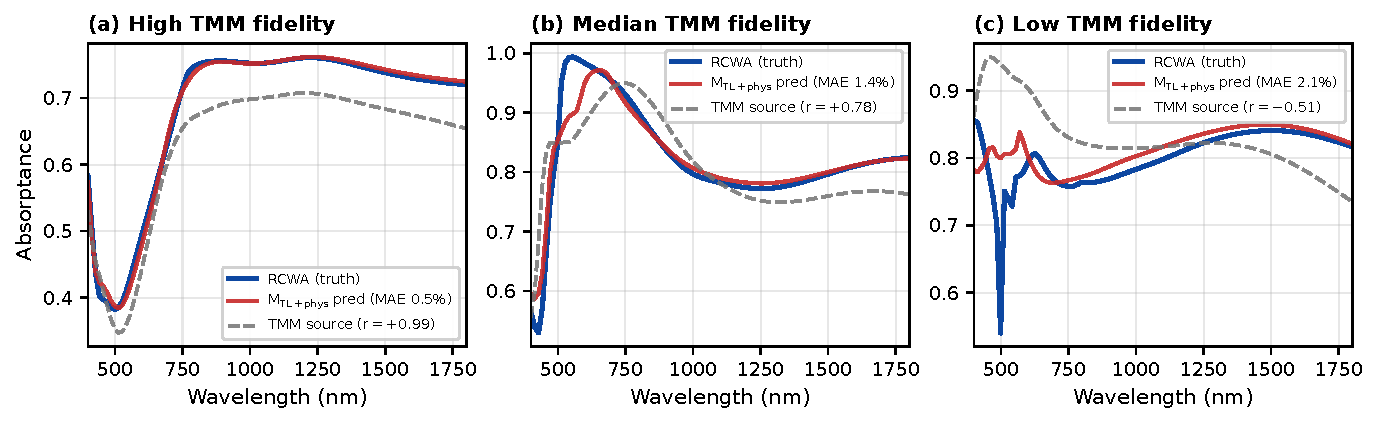
\includegraphics[width=\textwidth]{figures/Figure_S1.pdf}
\caption{Fine-tuned surrogate ($\Mtlphys$, Structure~A, $n=350$) predicted absorptance vs.\ RCWA ground truth for representative test geometries spanning high, median, and low TMM--RCWA fidelity (per-sample shape correlation $r$ indicated). The fine-tuned surrogate tracks the full-wave RCWA closely (per-sample MAE $0.5$--$2.1\%$ for these representative geometries) even where the TMM pre-training source (dashed) diverges from RCWA, confirming that fine-tuning on RCWA labels corrects the source's amplitude error.}
\label{fig:s1_surrogate_pred}
\end{figure}

\begin{figure}[htbp]\centering
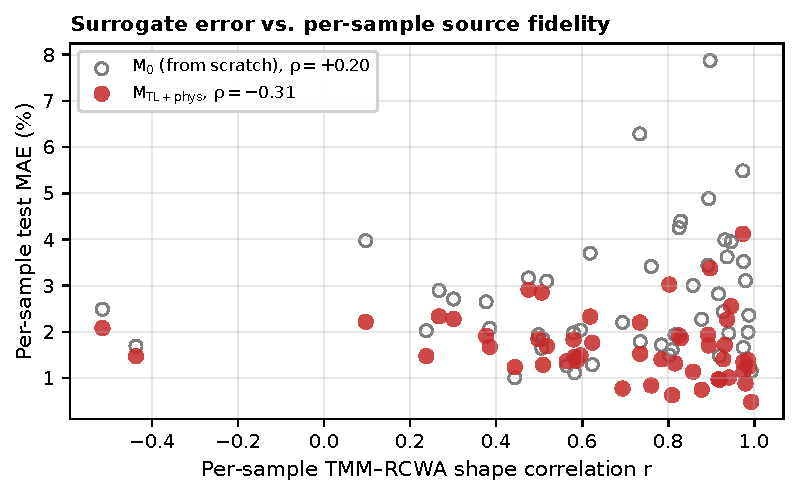
\includegraphics[width=0.62\textwidth]{figures/Figure_S2.pdf}
\caption{Per-sample surrogate test MAE vs.\ per-sample TMM--RCWA shape correlation $r$ (Structure~A, $50$ test geometries at $n=350$). The fine-tuned $\Mtlphys$ error is only weakly related to the per-sample source fidelity (Spearman $\rho=-0.31$) and is below the from-scratch $\Mzero$ for $44$ of the $50$ test geometries (median $1.5\%$ vs.\ $2.3\%$): the source-fidelity dependence of PBTL lives in the \emph{aggregate} weight-transfer benefit, not in a per-test-point error penalty.}
\label{fig:s2_error_vs_r}
\end{figure}

\begin{figure}[htbp]\centering
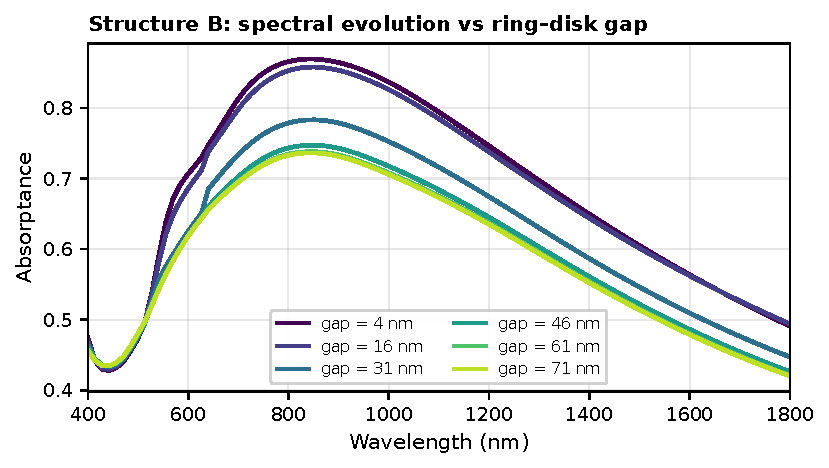
\includegraphics[width=0.7\textwidth]{figures/Figure_S3.pdf}
\caption{Structure~B (ring--disk) RCWA absorptance as the ring--disk gap is varied (disk radius swept at fixed ring geometry). The absorption resonance weakens monotonically as the gap widens (peak absorptance $0.87\to0.74$), supporting the interpretation that the Structure-B response arises from ring--disk near-field coupling. The sweep varies the disk radius, so it probes the coupled response rather than the gap in isolation.}
\label{fig:s3_gap_sweep}
\end{figure}

\begin{figure}[htbp]\centering
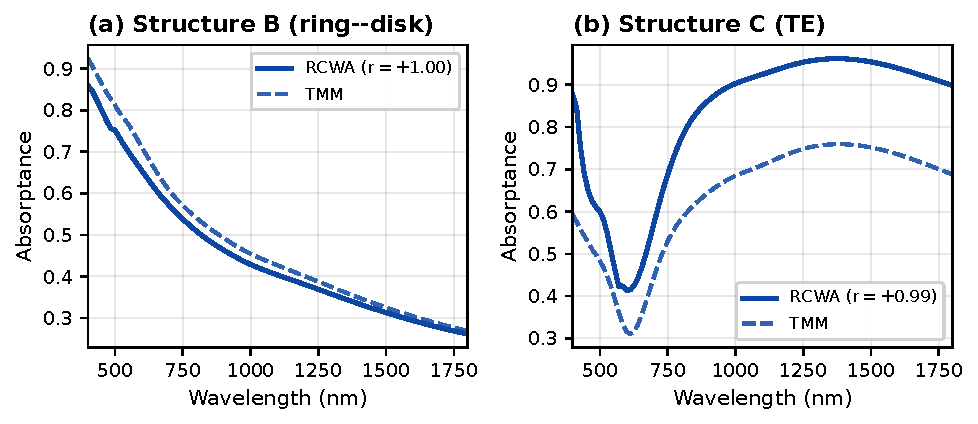
\includegraphics[width=\textwidth]{figures/Figure_S4.pdf}
\caption{Representative high-fidelity TMM (dashed) vs.\ RCWA (solid) absorptance spectra for Structures~B and~C (Structure~B by highest per-sample $r$; Structure~C the TE-polarized channel, selected by highest TE-only $r$), illustrating the cavity-like responses that the planar TMM source captures where its fidelity is high.}
\label{fig:s4_repr_spectra}
\end{figure}

% ============================================================
\clearpage
\section{Correction Change-Log}
\label{sec:si_changelog}
% ============================================================

While preparing the response to Reviewer~\#1, the convergence comment (point M7)
prompted a full audit of the forward-simulation pipeline. The audit identified
four corrections; because two of them required rebuilding the simulation data, we
regenerated the complete RCWA dataset for all three structures (A, B, C) and re-ran
every downstream analysis. Table~\ref{tab:si_changelog} catalogues the corrections,
and Table~\ref{tab:si_table1_corrected} reports the corrected Table~I
(TMM--RCWA spectral fidelity) against the submitted values. The optical-constant
correction is the dominant driver of the change.

\begin{table}[htbp]\centering\small
\caption{The four corrections applied during the pre-decision audit.}
\label{tab:si_changelog}
\begin{tabular}{p{0.30\linewidth} p{0.62\linewidth}}\toprule
\textbf{Correction} & \textbf{Description}\\\midrule
(1) Fourier convergence \newline (requested, M7) &
Under-converged truncation ($N=5$) replaced by per-wavelength adaptive orders up
to $N=17$ (raised by a feature-size/anisotropy heuristic; $N=17$ is the practical
memory ceiling, Sec.~\ref{sec:si_convergence}); the reported surrogate MAE is
dominated by network error rather than RCWA truncation, with any residual applied
identically across model variants.\\[0.4em]
(2) Optical constants \newline (independent) &
Tabulated Cr/Ti/Au extinction coefficients were inconsistent with the cited
Johnson \& Christy source (off by ${\sim}40$--$70\%$, up to ${\sim}36$\,pp
absorption impact in some regimes); rebuilt on measured Johnson \& Christy
constants (metals) and Siefke constants (TiO$_2$); both source datasets are cited
in the main-text Methods (``Optical constants''). \emph{Dominant driver of the
Table~I change.}\\[0.4em]
(3) Wavelength-grid fix \newline (independent) &
The Table~I fidelity script compared TMM and RCWA spectra on mismatched
wavelength grids; corrected to each structure's native grid, with Structure~A
unified to the broadband 400--1800\,nm convention used for B and C.\\[0.4em]
(4) Structure-C bounds \newline (independent) &
The $W_x/W_y$ normalization bounds were [50, 400]\,nm, narrower than the declared
design space ([50, 720]\,nm); 52\% of Structure-C samples normalized outside
$[0,1]$ and the TMM pre-training library under-covered the design space. Bounds
corrected to the declared range and all Structure-C results re-run; the
weight-transfer benefit grows from $+4\%$ to $+9.7\%$ at $n=350$.\\\bottomrule
\end{tabular}
\end{table}

\begin{table}[htbp]\centering\small
\caption{Corrected Table~I (TMM--RCWA spectral fidelity), submitted vs.\
corrected. ``Median $r$'' is the median per-sample shape correlation; ``TMM MAE''
is the operating-band absolute error. Values reflect all corrections jointly; the
optical-constant fix dominates.}
\label{tab:si_table1_corrected}
\begin{tabular}{lcccc}\toprule
\textbf{Structure} & \textbf{Median $r$ (subm.)} & \textbf{Median $r$ (corr.)} & \textbf{TMM MAE (subm.)} & \textbf{TMM MAE (corr.)}\\\midrule
A & $+0.72$ & $+0.83$ & $15.0\%$ & $7.9\%$\\
B & $-0.07$ & $+0.96$ & $27.0\%$ & $8.9\%$\\
C & $+0.34$ & $+0.65$ & $21.3\%$ & $16.9\%$\\\bottomrule
\end{tabular}
\end{table}

\paragraph{Impact on the conclusions.} These corrections do more than rescale
magnitudes, and we state the effect plainly. On the corrected data, the central
contribution---the fidelity--benefit diagnostic---continues to be supported,
though the supporting evidence changed: across the three corrected structures the
weight-transfer benefit forms a monotone gradient ($A>B>C$) that is ordered by the
operating-band absolute MAE rather than by shape correlation $r$ (the median-$r$
ordering $B>A>C$ mis-ranks the benefit). We note this is a cross-structure
ordering over only $N{=}3$ points (cross-structure linear correlation $|r|=0.61$),
complemented by a single-structure controlled noise sweep; we do not claim the
original conclusions carried through the corrections unchanged. One qualitative conclusion has changed:
on the corrected data Structures~B and C no longer show natural negative
weight-level transfer---both are positive at every training-set size---so the
original ``two distinct negative-transfer failure modes'' taxonomy has no empirical
support and has been \emph{removed} from the manuscript. Negative transfer is
retained solely as a \emph{controlled} result: degrading the TMM source toward zero
fidelity drives the benefit from $+47\%$ at full fidelity to $-58\%$ at zero
fidelity, a monotone fidelity--benefit relationship (Spearman $\rho=-1.0$) in which
the operating-band MAE predicts the benefit far better than the shape correlation
$r$ ($|r|=0.98$ vs.\ $0.81$ on the noise sweep; Sec.~\ref{sec:si_peng}).


\end{document}
